\documentclass{article}
\usepackage[utf8]{inputenc}
\usepackage{authblk}
\usepackage{natbib}
\usepackage{graphicx}
\usepackage{mathtools}                 % http://ctan.org/pkg/mathtools
\usepackage{amsmath}
\usepackage{listings}
\usepackage[a4paper, portrait, margin=1in]{geometry}

\usepackage[table]{xcolor}
\rowcolors{2}{gray!15}{white}
\newcommand{\head}[1]{%
   \textcolor{white}{\textbf{#1}}}
\renewcommand{\arraystretch}{1.5}

\title{\textbf{Analysis of 2-D Lid-Driven Cavity Problem}}
\author[1]{\textbf{Aakash Yadav}}
\affil[1]{\textbf{Indian Institute of Technology, Tirupati}}
\date{\textbf{April 2019}}
\geometry{a4paper, portrait, margin=1in}

\begin{document}
\maketitle

\begin{center}
\line(1,0){250}
\end{center}

\section{Introduction}
% literature review regarding the usage of this problem

\begin{figure}[h!]
\centering
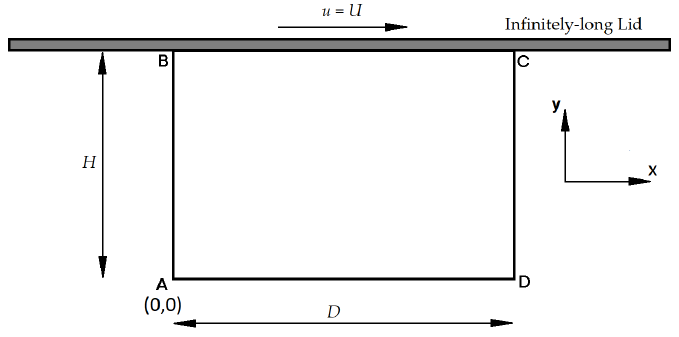
\includegraphics[scale=.5]{cavityFig.png}
\caption{scaling of the WF law by $A\left(r,\mu^*\right)$}
\label{fig:cavityFig}
\end{figure}

In this project, we will analyze the unsteady, viscous, incompressible,isothermal, two-dimensional, laminar flow of Newtonian fluid in a cavity covered with a lid. Consider a rectangular cavity ABCD of dimensions shown in Figure ~\ref{fig:cavityFig}. AB, CD, and AD are rigid walls, whereas BC is open. The cavity is of length $D$ and width $H$ , in the x-y plane, as shown in Figure 1.1. The aspect ratio is defined as $R=H/D$. The Reynolds number is defined based on the velocity scale $U$ and the length scale $D$. Acceleration due to gravity acts in the negative-z direction. The top of the cavity, BC, is covered with an infinitely-long rigid lid. Initially $(t \leq 0)$, the fluid inside the cavity is at rest. At time $t > 0$, the lid is set in motion to the right with a constant velocity $U $. You are to analyze the fluid flow inside the cavity for various conditions using proper governing equations, boundary conditions, initial conditions, and numerical schemes.
%
%In section 2, we bring out the corrections to the Wiedemann Franz law and form a generalised law. We further see how the corrective function varies with scattering parameter, $r$ and reduced chemical potential, $\mu^*$.
%In section 3,  we extremize the expression in form of the polylogarithmic functions for the thermal conductvity with respect to both reduced chemical potential, $\mu^*$ and temperature. We also present the mathematical approach to reduce the phonon thermal conductivity.
%Section 4 will provide an insight to mathematical form obtained by extremising the electrical conductivity with respect to temperature.
%In the final section we present the conclusions. 

\section{Governing Equations}
The Wiedemann Franz Law (1853) states that the ratio of the electronic contribution of the thermal conductivity $\kappa$ to the electrical conductivity $\sigma$ of a metal is proportional to the temperature $ T $ . \citep{Ashcroft}

Continuity equation for 2-D incompressible isothermal flow
\begin{equation}
\label{eqn:continuityEqn}
\frac{\partial u}{\partial x} + \frac{\partial v}{\partial y} = 0  
\end{equation}

Stream function 
\begin{equation}
\label{eqn:streamFnEqn}
\omega = -\left[\frac{\partial^2 \psi}{\partial x^2} +  \frac{\partial^2 \psi}{\partial y^2}\right]=-\nabla^2 \psi
\end{equation}

Navier-Stokes equations
\begin{equation}
\frac{\partial u}{\partial t} + u\frac{\partial u}{\partial x} + v\frac{\partial u}{\partial y}= -\frac{1}{\rho}\frac{\partial P}{\partial x} + g_x + \nu \left [ \frac{\partial^2 u}{\partial x^2} +  \frac{\partial^2 u}{\partial y^2} \right ]
\end{equation}

\begin{equation}
\frac{\partial v}{\partial t} + u\frac{\partial v}{\partial x} + v\frac{\partial v}{\partial y}= -\frac{1}{\rho}\frac{\partial P}{\partial y} + g_y + \nu \left [ \frac{\partial^2 v}{\partial x^2} +  \frac{\partial^2 v}{\partial y^2} \right ]
\end{equation}

Vorticity relation 
\begin{equation}
\label{eqn:vorticityFnEqn}
\frac{\partial \omega_z}{\partial t} + u\frac{\partial \omega_z}{\partial x} + v\frac{\partial \omega_z}{\partial y}= \nu \left [ \frac{\partial^2 \omega_z}{\partial x^2} +  \frac{\partial^2 \omega_z}{\partial y^2} \right ]
\end{equation}
% \notag

Where, k is the Boltzmann constant, e is the electronic charge and the constant $L_0$ is  known as the Lorenz number.
For over 150 years, the Wiedemann Franz law has proven to be stable amongst the multitude of metallic systems that have been studied. 
But recent experiments over a couple of decades show that there are several limitations to the law, the value of Lorenz number L is not same for every materials and the law does not hold for intermediate temperatures. Experiments have shown that the value of Lorenz number, $L$, while roughly constant, is not exactly the same for all materials. 
 \citep{Bristol,2017Sci...355..371L} 

\section{Courant–Friedrichs–Lewy anakysis}
In mathematics, the Courant–Friedrichs–Lewy (CFL) condition is a necessary condition for convergence while solving certain partial differential equations (usually hyperbolic PDEs) numerically. It arises in the numerical analysis of explicit time integration schemes, when these are used for the numerical solution. As a consequence, the time step must be less than a certain time in many explicit time-marching computer simulations, otherwise the simulation produces incorrect results. The condition is named after Richard Courant, Kurt Friedrichs, and Hans Lewy who described it in their 1928 paper.
 We have the 

\section{Initial Conditions and Boundary Conditions}

At time $t=0$ everything is at rest and hence all the values are zero. At the moment $t \geq0$ the lid will be moving at speed $u=U$, which will try to set the fluidin motion. We have the following boundary conditions for $t\geq0$ :
\\*
No slip condition will result in zero velocity along the wall tangent
\begin{subequations}
\begin{equation}
u(x,0)=0
\end{equation}
\begin{equation}
v(D,y)=0
\end{equation}
\begin{equation}
u(x,H)=U
\end{equation}
\begin{equation}
u(0,y)=0
\end{equation}
\end{subequations}
\\*
The no penetration condition that the walls of the cavity are impervious results into
\begin{subequations}
\begin{equation}
v(x,0)=0
\end{equation}
\begin{equation}
u(D,y)=0
\end{equation}
\begin{equation}
v(x,H)=0
\end{equation}
\begin{equation}
u(0,y)=0
\end{equation}
\end{subequations}


\section{Non-dimensionalization of the Governing Equations}
% comment on normalization	
It is convenient numerically to make the equations for y and w dimensionless. This means we need to introduce the appropriate scalings for the dimensionless variables.
\begin{equation}
\hat{x}=\frac{x}{D}, \hat{y}=\frac{y}{H},  \hat{t}=\frac{U}{D}t,  \hat{u}=\frac{u}{U},  \hat{v}=\frac{v}{V_{ref}}
\end{equation}
\\*
Non-dimensionalising Equation \ref{eqn:continuityEqn} results into 
\begin{subequations}
\begin{equation}
\frac{U}{D}\frac{\partial \hat{u}}{\partial \hat{x}} + \frac{V_{ref}}{H}\frac{\partial \hat{v}}{\partial \hat{y}} = 0  
\end{equation}
\begin{equation}
\frac{U}{D}\sim \frac{V_{ref}}{H}  
\end{equation}
\begin{equation}
V_{ref}= \left(\frac{H}{D}\right)U = RU  
\end{equation}
\end{subequations}

\begin{equation}
\hat{\psi}=\frac{\psi}{UD},  \hat{\omega}=\frac{\omega D}{U}
\end{equation}
\\*
Non-dimensionalising the stream function equation (\ref{eqn:streamFnEqn})
\begin{subequations}
\begin{equation}
\frac{\hat{\omega} U}{D} = -\left[\frac{\partial^2 (\hat{\psi}UD)}{\partial (\hat{x}D)^2} +  \frac{\partial^2 (\hat{\psi UD)}}{\partial (\hat{y}H)^2}\right]
\end{equation}
\begin{equation}
\label{eqn:streamFnEqn3}
\hat{\omega} = -\left[\frac{\partial^2 \hat{\psi}}{\partial \hat{x}^2} +  \frac{1}{r^2}\frac{\partial^2 \hat{\psi}}{\partial \hat{y}^2}\right]
\end{equation}
\end{subequations}
\\*
Non-dimensionalising the vorticity function equation (\ref{eqn:vorticityFnEqn})
\begin{subequations}
\begin{equation}
\frac{\partial \left(\frac{U}{D}\hat{\omega_z}\right)}{\partial \left(\frac{D}{U}\hat{t}\right)} + \hat{u}U\frac{\partial \left(\frac{U}{D}\hat{\omega_z}\right)}{\partial (\hat{x}D)} + \frac{UH}{D}\hat{v}\frac{\partial \left(\frac{U}{D}\hat{\omega_z}\right)}{\partial (\hat{y}H)}= \nu \left [ \frac{\partial^2 \left(\frac{U}{D}\hat{\omega_z}\right)}{\partial (\hat{x}D)^2} +  \frac{\partial^2 \left(\frac{U}{D}\hat{\omega_z}\right)}{\partial (\hat{y}H)^2} \right ]
\end{equation}
\begin{equation}
\label{eqn:vorticityEqn2}
\frac{\partial \hat{\omega_z}}{\partial \hat{t}} + \hat{u}\frac{\partial \hat{\omega_z}}{\partial \hat{x}} + \hat{v}\frac{\partial \hat{\omega_z}}{\partial \hat{y}}= \frac{\nu}{UD} \left [ \frac{\partial^2 \hat{\omega_z}}{\partial \hat{x}^2} +  \frac{1}{r^2}\frac{\partial^2 \hat{\omega_z}}{\partial \hat{y}^2} \right ]
\end{equation}
\end{subequations}
Also we have 
\begin{equation}
\label{eqn:vorticityEqn3}
u=\frac{\partial \psi}{\partial y} , v=-\frac{\partial \psi}{\partial x}
\end{equation}
\\*
Non-dimensionalisation of the above equation results into
\begin{equation}
\label{eqn:streamFnEqn2}
\hat{u}=\frac{1}{r}\frac{\partial \hat{\psi}}{\partial \hat{y}} , \hat{v}=-\frac{1}{r}\frac{\partial \hat{\psi}}{\partial \hat{x}}
\end{equation}
Substituting equation (\ref{eqn:vorticityEqn3}) in equation (\ref{eqn:vorticityEqn2}) yields 
\begin{equation}
\label{eqn:vorticityEqn4}
\frac{\partial \hat{\omega_z}}{\partial \hat{t}} +\frac{1}{r}\left[\frac{\partial \hat{\psi}}{\partial \hat{y}}\frac{\partial \hat{\omega_z}}{\partial \hat{x}} - \frac{\partial \hat{\psi}}{\partial \hat{x}}\frac{\partial \hat{\omega_z}}{\partial \hat{y}}\right]= \frac{1}{Re} \left [ \frac{\partial^2 \hat{\omega_z}}{\partial \hat{x}^2} +  \frac{1}{r^2}\frac{\partial^2 \hat{\omega_z}}{\partial \hat{y}^2} \right ]
\end{equation}
where, $Re = \frac{UD}{\nu}$
\\*
Deriving the boundary conditions in the form of vorticity
\begin{subequations}
\begin{equation}
\hat{\omega}(\hat{x},0) = - \frac{1}{r^2}\left(\frac{\partial^2 \hat{\psi}}{\partial \hat{y}^2}\right)_{\hat{y}=0}
\end{equation}
\begin{equation}
\hat{\omega}(\hat{x},1) = - \frac{1}{r^2}\left(\frac{\partial^2 \hat{\psi}}{\partial \hat{y}^2}\right)_{\hat{y}=1}
\end{equation}
\begin{equation}
\hat{\omega}(0,\hat{y}) = -\left(\frac{\partial^2 \hat{\psi}}{\partial \hat{x}^2}\right)_{\hat{x}=0}
\end{equation}
\begin{equation}
\hat{\omega}(1,\hat{y}) = -\left(\frac{\partial^2 \hat{\psi}}{\partial \hat{x}^2}\right)_{\hat{x}=1}
\end{equation}
\end{subequations}

Deriving the boundary conditions in the form of vorticity. For the bottom surface $\hat{u}=\hat{v}=0$, substituiting this equation (\ref{eqn:streamFnEqn2}) yields 
\begin{equation}
\hat{\psi}_{(\hat{y}=0)} = c_1
\end{equation}
Where $c_1$ is the integration constant. Similarly we can obtain the equations for the other walls as
\begin{equation}
\hat{\psi}_{(\hat{x}=0)} = c_2, \hat{\psi}_{(\hat{x}=1)} = c_3 
\end{equation}
For the top wall
\begin{equation}
\hat{u} = U =  \frac{1}{r}\frac{\partial \hat{\psi}}{\partial \hat{y}}  \Rightarrow \hat{\psi} = rUH+c_4  =c_5
\end{equation}
\begin{equation}
\hat{\psi}_{(\hat{y}=1)} = c_5
\end{equation}

\begin{figure}[h!]
\centering
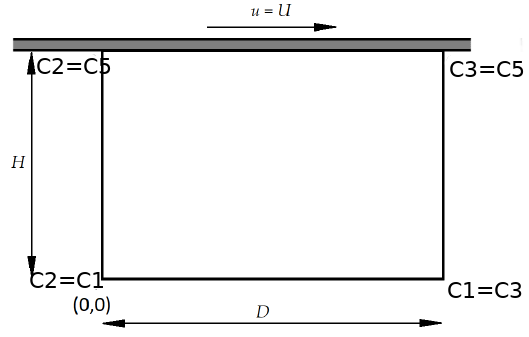
\includegraphics[scale=.4]{cavityFig2.png}
\caption{scaling of the WF law by $A\left(r,\mu^*\right)$}
\label{fig:cavityFig2}
\end{figure}

We have $c_1=c_2=c_3=c_5=c$ because of the continuity at the corners as shown in the Figure \ref{fig:cavityFig2}. Without any loss of generality we can set $c=0$ as $\psi$ is a relative term.
Hence
\begin{equation}
\hat{\psi}_{(y=0)}=\hat{\psi}_{(y=1)}=\hat{\psi}_{(x=0)}=\hat{\psi}_{(x=1)}=0
\end{equation}




\section{ Discretization Schemes}
% comment why do we use such a grid with a stretching function --> velocity gradient is hight near walls. Why only that particular stretching function

\begin{figure}[h!]
\centering
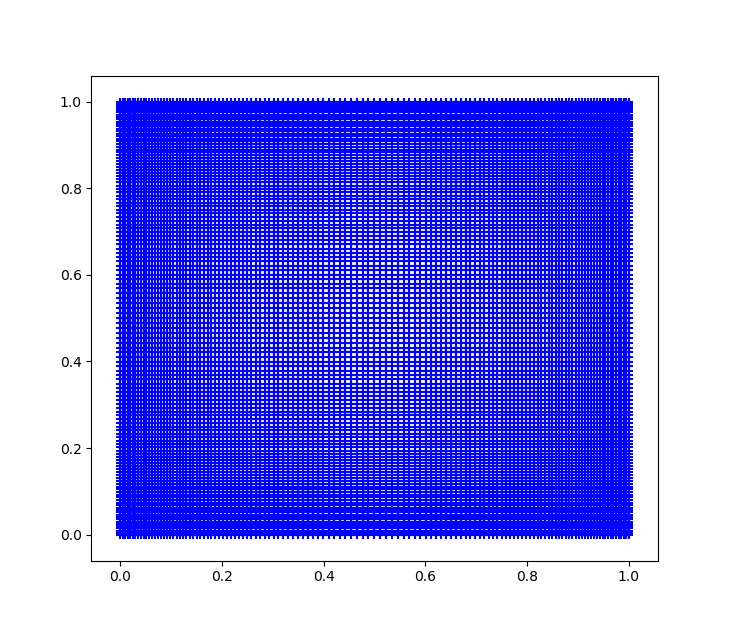
\includegraphics[scale=.5]{Figure_1.png}
\caption{A 128 $\times$ 128 grid generated by the program}
\label{fig:gridImage}
\end{figure}
In the analysis that follows we will drop the 'hat' notation for dimensionless variables for convienance. We will first use the usual FTCS scheme and a grid that is not equally spaced as shown in Figure \ref{fig:gridImage}. Derive the orders of accuracies of this scheme for both time and space. The values of $\Delta x$ and $\Delta y$ are not constant. You must use an appropriate stretching function so that the number of grid points vary in such a way that more grid points are concentrated closer to walls and the lid. Why is this necessary? Comment on this! Do a Von-Neumann stability analysis to find out the CFL criterion and the maximum time step to be used in your calculations. You may notice that $\Delta x,\Delta y,u,v$ are going to vary throughout the domain. So, the grid Courant number is also going to vary for every node, and every time step. So your code/program/algorithm must be adaptive; i.e, it must be able to choose the correct values of $\Delta t$ so that the CFL criterion is satisfied at all times and at all locations in the domain.
\\*
Discretiztion of equation \ref{eqn:streamFnEqn3} using forward time and central differencing scheme. Second order accurate in space.
\begin{equation}
\frac{\psi_{i+1,j}-2\psi_{i,j}+\psi_{i-1,j} }{(\Delta x)^2} + \frac{1}{r^2}\frac{\psi_{i,j+1}-2\psi_{i,j}+\psi_{i,j-1}}{(\Delta y)^2} = -\omega_{zij}
\end{equation}
Von-Newmann stability analysis for the above equation -
\\*
Discretiztion of equation \ref{eqn:vorticityEqn4}  using forward time and central differencing scheme. First order time accurate and second order space accurate. 
\begin{equation} 
\begin{split}
\frac{\omega_{i,j}^{n+1}-\omega_{i,j}^{n}}{\Delta t}+\frac{1}{r}\left[\left(\frac{\psi_{i,j+1}-\psi_{i,j-1}}{2\Delta y}\right)\left(\frac{\omega_{i+1,j}-\omega_{i-1,j}}{2\Delta x}\right) - \left(\frac{\psi_{i+1,j}-\psi_{i-1,j}}{2\Delta x}\right)\left(\frac{\omega_{i,j+1}-\omega_{i,j-1}}{2\Delta y}\right)  \right] \\
  = \frac{1}{Re}\left[\left(\frac{\omega_{i+1,j}-2\omega_{i,j}+\omega_{i-1,j}}{(\Delta x)^2}\right)+\frac{1}{r^2}\left(\frac{\omega_{i,j+1}-2\omega_{i,j}+\omega_{i,j-1}}{(\Delta y)^2}\right) \right]
\end{split}
\end{equation}
Von-Neutmann stability analysis for the above equation -
% von newmann stability is only valid for linear equation, so check if the above equation is linear
% we will be using adaptive time marching scheme for this

\section{Algorithm}
\begin{table}[ht]
   \centering
   \sffamily
   \begin{tabular}{rlr}
     \rowcolor{black!75}
      \head{No.}& \head{Steps}  \\
     1 & Initialize $u$ and $v$ values        \\
     2 & Define the vorticity equation    \\
     3 & Solve Poisson equation for stream function    \\
     4 & Solve vorticity transport equation at a forward time step $t+\Delta t$ \\
     5 & Solve the Poisson equation for stream function at  $t+\Delta t$   \\
     6 & Find $u$ and $v$ using the vorticity function equation      \\
     7 & Check if the CFL criteria is satisified, if yes proced to next step     \\
     8 & Else change the time step size and repeat the loop     \\
  \end{tabular}
\end{table}


The Fermi-Dirac integrals play very improtant role in the study of semiconductors appear frequently in semiconductor problems. It is thus a topic of special interest among physicist working in this field.

\section{Results}
% what is the Re at which turbulance starts and fluid shows transition i.e. vorticities
The Fermi-Dirac integrals play very improtant role in the study of semiconductors appear frequently in semiconductor problems. It is thus a topic of special interest among physicist working in this field.

\subsection{Grid Independence Studies}
The formulation for obtaining the minimum lattice thermal conductivity is given by approach developed by Cahill \citep{PhysRevB.46.6131}. To minimise the Phonon thermal conductivity, the integrand has been extremised and simplified yielding solution in the form of offset log function. The plot for the integrand essentially Planck's blackbody radiation function has also been shown in Figure 2.

\subsection{Streamlines for Varying R and Re}
The efficiency of the thermoelectric material is directly proportional to the electrical conductivity of the material. Maximizing the same is of the utmost importance inorder to increase its efficiency. We have the following expression for the electrical . \citep{articleSRV}


\subsection{Profiles for Steady Flow}

Exact Fermi Dirac Integral expressions can be very helpful in generalizing the Wiedemann Franz  Law. 

\section{Discussion}

Exact Fermi Dirac Integral expressions can be very helpful in generalizing the Wiedemann Franz  Law. Exact analytic expressions of the same will greatly assist and equip the researchers in the new material design processes.  Electronic thermal conductivity, $\kappa_e$ and minimum lattice thermal conductivity $\kappa_{l,min}$  have exact analytic expressions and we have obtained very interesting forms of solutions while maximising the two. More recent observations on the influence of anharmonicity on  $\kappa_{l,min}$  suggest that the Polylogarithms and Lambert W can have more interesting applications.

\section*{Appendix}
The below code can be used for plotting the scaling factor A as shown in Figure 1.
\lstinputlisting{gridGen.py}

\bibliographystyle{plain}
\bibliography{references}
\end{document}

